%==============================================================================
\chapter{Ergebnisse} \label{chap:ergebnis}
%==============================================================================

In diesem Kapitel werden mit der vorgeschlagenen Modellierung von Kraftstoffsystemen für Fluggasturbinen berechnete Ergebnisse analysiert. Dabei steht insbesondere die Frage im Fokus, ob die Modellierung den Leistungs- und Wärmebedarf der Kraftstoffsysteme akkurat vorhersagen kann. Zunächst wird in einer Sensitivitätsanalyse die Auswirkung von Unsicherheiten der in Kapitel \ref{chap:param} bestimmten Parametern auf das Modellverhalten untersucht. Danach wird die Methodik dieser Arbeit daher mit Daten aus der Literatur validiert. Anschließend wird im Rahmen einer Parameterstudie analysiert, wie sich die Eintrittstemperaturen des Kraftstoffs in den Wärmeübertrager und die Brennkammer auf die Modellierungen der Wasserstoff-Kraftstoffsysteme auswirkt. Abschließend erfolgt ein Vergleich des Betriebsmittelbedarfs der H$_2$-Kraftstoffsysteme untereinander und mit dem Referenzkraftstoffsystem anhand eines ausgewählten Betriebspunkts.

\section{Sensitivitätsanalyse}

Im Folgenden wird eine Sensitivitätsanalyse durchgeführt und ausgewertet, um die für das Modellverhalten maßgeblichen Parameter zu identifizieren. Zunächst werden hierfür die Unsicherheiten der Parameter geschätzt. Anschließend werden die mit Unsicherheit behafteten Parameter in die Modellierungen der Kraftstoffsysteme eingesetzt, um die Abweichungen Leistungsbedarfe zu berechnen.

\subsection{Bestimmung der Schrittweiten}

Da die statistische Verteilung der Parameterwerte nicht bekannt ist, werden die Schrittweiten für die Variation der Parameter geschätzt. Die Schrittweiten werden so gewählt, dass die Abweichung der Pumpenleistung des H$_2$-Kraftstoffsystems mit Verdampfer stets ein positives Vorzeichen aufweist.

Der Austrittsdruck der Niederdruckpumpe $p_\mathrm{LPFP}$ des kerosinbetriebenen Kraftstoffsystems ist stets höher als der Öldruck im Wärmeübertrager des Hauptölsystems und somit von diesem abhängig. Der Öldruck ist eine Funktion der Druckverlust des Ölsystems. Aus diesem Grund wird eine moderate Schrittweite von $-10\,\%$ gewählt.

Da die Druckverluste von Wärmeübertragern und Leitungen ein Auslegungsziel darstellen, sind sie nicht direkt mit Unsicherheit behaftet. Jedoch können abweichende Anforderungen an das Gewicht dieser Komponenten eine Aufweichung der Auslegungsziele erfordern. Um diesen Effekt zu berücksichtigen werden der Leitungsdruckverlust $\Delta p_L$ und die Druckverluste $1-\pi_i$ der Wärmeübertrager mit einer Schrittweite von $+20\,\%$ variiert. 

Die Druckverluste des Verdampfers $1-\pi_{\mathrm{V}, i}$ werden in der Modellierung des Kraftstoffsystems vernachlässigt. Da auf der Hochdruckseite zwar geringe, jedoch im Verhältnis zur Niederdruckseite höhere Druckverluste zu erwarten sind (Siehe Kapitel \ref{chap:param}), werden absolute Schrittweiten von $+0,01$ auf der Hochdruckseite und $+0,005$ auf der Niederdruckseite verwendet. 

Die Unsicherheiten der Wirkungsgrade von Pumpen und Verdichtern $\eta_i$, der verfügbaren Abwärme $\dot{Q}_\mathrm{FOHE}$  und den Injektor-Druckverlusten $\Delta p_\mathrm{inj}$ werden als gering eingeschätzt. Aus diesem Grund wird für diese Parameter eine Schrittweite von $\pm 5\,\%$ ausgewählt.

\subsection{Auswertung der Sensitivitätsanalyse}

Auf Basis der zuvor bestimmten Schrittweiten wird im Folgenden die Sensitivität der Kraftstoffsysteme untersucht und ausgewertet. Zunächst werden die Ergebnisse der Modellierung des H$_2$-Kraftstoffsystems mit Verdampfer präsentiert. Daraufhin werden die Ergebnisse der Sensitivitätsanalysen der H$_2$-Kraftstoffsysteme miteinander verglichen. Abschließend werden die Ergebnisse der Sensitivitätsanalyse für das kerosinbetriebene Kraftstoffsystem diskutiert.

Die Ergebnisse der Sensitivitätsanalyse für das H$_2$-Kraftstoffsystem mit Verdampfer sind in Tabelle \ref{Tab:sensjeta} dargestellt.

\begin{table}[ht]
	\centering
	\caption{Sensitivitätsanalyse des H$_2$-Kraftstoffsystems mit Verdampfer}
	\begin{tabular} {|l|c|c|c|c|c|} \hline%
		Parameter & Einheit & Schrittweite & Schrittweite [\%] & $ \Delta \sum P_i$ [\%] \\ \hline\hline%
		$\Delta p_\mathrm{L}$ & \si{\kilo\Pa} & +52,0 & +20,0 & +5,39 \\ \hline 
		$1-\pi_\mathrm{FOHE}$ & - & +0,010 & +20,0 & +1,98 \\ \hline 
		$1-\pi_\mathrm{PHC}$ & - & +0,004 & +20,0 & +0,768 \\ \hline
		$\eta_\mathrm{HPFC}$ & - & -0,0355 & -5,00 & +2,68 \\ \hline  
		$\eta_\mathrm{RV}$ & - & -0,0355 & -5,00 & +1,71 \\ \hline 
		$\dot{Q}_\mathrm{FOHE}$ & \si{\kilo\W} & -7,95 & -5,00 & +0,0541 \\ \hline 
		$\Delta p_\mathrm{inj}$ & \si{\kilo\Pa} & +8,45 & +5,00 & +0,0829 \\ \hline 
		$1-\pi_\mathrm{V, HP}$ & - & +0,010 & - & +1,88 \\ \hline 
		$1-\pi_\mathrm{V, LP}$ & - & +0,005 & - & +0,202 \\ \hline 
	\end{tabular}	
	\label{Tab:sensafter}%
\end{table}
\FloatBarrier 

Mit einem Anstieg der Leistungen um  $+5,39\,\%$ hat die Erhöhung der Leitungs-Druckverluste bei Weitem die größte Auswirkung auf die Modellierung des H$_2$-Kraftstoffsystems mit Verdampfer. Die Reduktionen der Wirkungsgrade der Verdichter haben mit $+2,68\,\%$ (Hochdruckverdichter) beziehungsweise $+1,71\,\%$ (Rezirkulationsverdichter) nur eine moderate Auswirkung auf die Verdichterleistungen. 

Die Erhöhungen der Druckverluste des Ölsystem-Wärmeübertragers und der Hochdruckseite des Verdampfers führen mit $1,98\,\%$ und $1,88\,\%$ ebenfalls zu moderaten anstiegen der Leistungen. Hingegen hat der Anstieg der Druckverluste des PHC-Wärmeübertragers und der Niederdruckseite des Verdampfers nur geringen Einfluss auf die Leistungen. 

Ein Anstieg der Injektor-Druckverluste hat nur geringe Auswirkungen auf die Verdichter-Leistungen.


Die Tabellen \ref{Tab:senspump} und \ref{Tab:sensdual} zeigen die Ergebnisse der Sensitivitätsanalysen für die H$_2$-Kraftstoffsysteme mit Hochdruckpumpe und Vormischung.

\begin{table}[ht]
	\centering
	\caption{Sensitivitätsanalyse des H$_2$-Kraftstoffsystems mit Pumpe}
	\begin{tabular} {|l|c|c|c|c|c|} \hline%
		Parameter & Einheit & Schrittweite & Schrittweite [\%] & $ \Delta \sum P_i$ [\%] \\ \hline\hline%
		$\Delta p_\mathrm{L}$ & \si{\kilo\Pa} & +52,0 & +20,0 & +8,19 \\ \hline 
		$1-\pi_\mathrm{FOHE}$ & - & +0,010 & +20,0 & +3,01 \\ \hline 
		$1-\pi_\mathrm{PHC}$ & - & +0,004 & +20,0 & +1,17 \\ \hline
		$\eta_\mathrm{HPFP}$ & - & -0,0077 & -5,00 & +1,41 \\ \hline  
		$\eta_\mathrm{RV}$ & - & -0,0355 & -5,00 & +2,96 \\ \hline 
		$\dot{Q}_\mathrm{FOHE}$ & \si{\kilo\W} & -7,95 & -5,00 & +0,055 \\ \hline 
		$\Delta p_\mathrm{inj}$ & \si{\kilo\Pa} & +8,45 & +5,00 & -0,0523 \\ \hline 
	\end{tabular}	
	\label{Tab:senspump}%
\end{table}
\FloatBarrier 

\begin{table}[ht]
	\centering
	\caption{Sensitivitätsanalyse des H$_2$-Kraftstoffsystems mit Vormischung}
	\begin{tabular} {|l|c|c|c|c|c|} \hline%
		Parameter & Einheit & Schrittweite & Schrittweite [\%] & $ \Delta \sum P_i$ [\%] \\ \hline\hline%
		$\Delta p_\mathrm{L}$ & \si{\kilo\Pa} & +52,0 & +20,0 & +5,38 \\ \hline 
		$1-\pi_\mathrm{FOHE}$ & - & +0,010 & +20,0 & +1,97 \\ \hline 
		$1-\pi_\mathrm{PHC}$ & - & +0,004 & +20,0 & +0,766 \\ \hline
		$\eta_\mathrm{HPFC}$ & - & -0,0355 & -5,00 & +2,68 \\ \hline  
		$\eta_\mathrm{RV}$ & - & -0,0355 & -5,00 & +1,70 \\ \hline 
		$\dot{Q}_\mathrm{FOHE}$ & \si{\kilo\W} & -7,95 & -5,00 & +0,0551 \\ \hline 
		$\Delta p_\mathrm{inj}$ & \si{\kilo\Pa} & +8,45 & +5,00 & +0,0838 \\ \hline 
	\end{tabular}	
	\label{Tab:sensdual}%
\end{table}
\FloatBarrier 

Die H$_2$-Kraftstoffsysteme weisen nur geringfügige Unterschiede in ihren Sensitivitäten auf. Das H$_2$-Kraftstoffsystem mit Hochdruckpumpe zeigt mit $+8,19\,\%$ eine besonders hohe Sensitivität gegenüber Variationen der Leitungs-Druckverluste. Auch Änderungen der Druckverluste in den Wärmeübertragern haben einen stärkeren Einfluss auf dieses System. Die Ergebnisse des H$_2$-Kraftstoffsystems mit Vormischung weichen nur minimal von denen des H$_2$-Kraftstoffsystems mit Verdampfer ab.

Die Ergebnisse der Sensitivitätsanalyse für das kerosinbetriebene Kraftstoffsystem sind in Tabelle \ref{Tab:sensjeta} zusammengefasst.

\begin{table}[ht]
	\centering
	\caption{Sensitivitätsanalyse des kerosinbetriebenen Kraftstoffsystems}
	\begin{tabular} {|l|c|c|c|c|} \hline%
		Parameter & Einheit & Schrittweite & Schrittweite [\%] & $ \Delta \sum P_i$ [\%] \\ \hline\hline%
		$p_\mathrm{LPFP}$ & - & -93,0 & -10,0 & +4,38 \\ \hline 
		$\Delta p_\mathrm{L}$ & \si{\kilo\Pa} & +13,6 & +20,0 & +1,21 \\ \hline 
		$1-\pi_\mathrm{FOHE}$ & - & +0,010 & +20,0 & +0,828 \\ \hline 
		$\eta_\mathrm{HPFP}$ & - & -0,0365 & -5,00 & +3,81 \\ \hline 
		$\eta_\mathrm{LPFP}$ & - & -0,030 & -5,00 & +1,48 \\ \hline 
		$\dot{Q}_\mathrm{FOHE}$ & \si{\kilo\W} & -6,35 & -5,20 & -1,36 \\ \hline 
		$\Delta p_\mathrm{inj}$ & \si{\kilo\Pa} & +30,0 & +10,0 & +2,67 \\ \hline 
	\end{tabular}	
	\label{Tab:sensjeta}%
\end{table}
\FloatBarrier 

Zwar führt der verringerte Austrittsdruck zu einer geringeren Leistung der Niederdruckpumpe, jedoch steigt hierdurch das Druckverhältnis und die Leistung der Hochdruckpumpe. Die Auswirkungen auf die Hochdruckpumpe überwiegen, was zu einem Anstieg des Leistungsbedarfs um $4,38\,\%$ führt – der größten Abweichung unter den Parametern. 

Eine Verringerung des Wirkungsgrads der Hochdruckpumpe hat einen um $3,81\,\%$ höheren Leistungsbedarf zur Folge. Aufgrund des geringeren Leistungsbedarfs der Niederdruckpumpe hat die Variation ihres Wirkungsgrads mit $1,48\,\%$ eine geringere Auswirkung. 

Eine Steigerung der Injektor-Druckverluste führt zu einem um $2,67\,\%$ höheren Leistungsbedarf der Pumpen. Im Vergleich haben die Variation der Leitungs- und Wärmeübertrager-Druckverluste einen geringen Einfluss auf den Leistungsbedarf. 

Die kleinere Abwärme führt zu einem geringeren Massenstrom durch die Niederdruckpumpe und somit zu einer um $1,36\,\%$ verringerten Pumpenleistung.

\section{Validierung}

Zur Validierung der Methodik dieser Arbeit wird das Wasserstoff-Kraftstoffsystem mit Pumpe angepasst und parametriert, um das von Brewer \cite{Brewer.1991} vorgeschlagene Kraftstoffsystem nachzuempfinden. 

Dabei werden folgende Modifikationen an der Modellierung vorgenommen: Die Druckverluste im rezirkulierten Kraftstoffstrom werden vernachlässigt, da das Kraftstoffsystem nach Brewer keinen Rezirkulationsverdichter vorsieht. Der Kraftstoffmassenstrom wird nicht an die Brennkammer-Eintrittstemperatur angepasst und eine parallele Wasserstoffverbrennung ist nicht vorgesehen. Zudem bleibt der Wärmeeintrag des von Brewer vorgeschlagenen Rekuperators unberücksichtigt, da sich dieser Wärmeübertrager Stromabwärts der Entnahmestelle des rezirkulierten Kraftstoffs befindet - eine Konfiguration, die von der Modellierung dieser Arbeit abweicht. Um dennoch eine Vergleichbarkeit der Pumpenleistung zu gewährleisten, wird der Druckverlust dieses Wärmeübertragers zu den Druckverluste der Injektoren addiert. 

Ein weiterer Unterschied liegt in der Modellierung des Kraftstoffs: Während in dieser Arbeit Parawasserstoff verwendet wird, basieren Brewers Berechnungen auf Normalwasserstoff. Dies macht eine Anpassung der Modellparameter des Wasserstoff-Stoffmodels erforderlich. Tabelle \ref{Tab:brewer} zeigt die weiteren Änderungen der Parameter und Variablen gegenüber dem ursprünglichen Wasserstoff-Kraftstoffsystem mit Pumpe.

\begin{table}[ht]
    \centering
	\caption{Veränderte Parameter der Validierung}
	\begin{tabular} {|l|c|c|c|} \hline%
    \multicolumn{2}{|c|}{Parameter} & Einheit & Wert\\ \hline\hline%
    FOHE Druckverhältnis & $\pi_\mathrm{FOHE}$ & - & 1 \\ \hline
    Brennkammer-Massenstrom & $\dot{m}_\mathrm{BK}$ & kg/s & 0,166 \\ \hline
    Leitungsdruckverluste & $\Delta p_\mathrm{r}$ & kPa & 30 \\ \hline
    Injektordruckverluste & $\Delta p_\mathrm{inj}$ & kPa & 214,4 \\ \hline
    Brennkammer-Eintrittsdruck & $p_\mathrm{BK}$ & kPa & 1516,2 \\ \hline
    Brennkammer-Eintrittstemperatur & $T_\mathrm{BK}$ & K & 264 \\ \hline
    Wärmeübertrager-Eintrittstemperatur & $T_\mathrm{W}$ & K & 200 \\ \hline
    \end{tabular}	
    \label{Tab:brewer}%
\end{table}
\FloatBarrier 

Tabelle \ref{Tab:validation} zeigt die von Brewer berechneten Werte und die mit der beschriebenen Methodik berechneten Werte. 

\begin{table}[ht]
    \centering
	\caption{Validierung der Methodik}
	\begin{tabular} {|l|c|c|c|c|} \hline%
    \multicolumn{2}{|c|}{Variable} & Einheit & Brewer \cite{Brewer.1991} & Diese Arbeit \\ \hline\hline%
    Pumpenleistung & $P_\mathrm{HPFP}$ & kW & 23,9 & 23,4 \\ \hline
    Wärme & $\dot{Q}$ & kW & 542,7 & 539,8 \\ \hline
    Rezirkulierter Massenstrom & $\dot{m}_\mathrm{R}$ & kg/s & 0,377 & 0,439 \\ \hline
    Pumpen-Austrittstemperatur & $T_{2,\mathrm{HPFP}}$ & K & 50 & 33,1 \\ \hline
    \end{tabular}	
    \label{Tab:validation}%
\end{table}
\FloatBarrier 

Die Werte für die Pumpenleistung und den Wärmebedarf stimmen weitgehend mit den Berechnungen von Brewer überein. Allerdings berechnet Brewers einen um $14\,\%$ geringeren rezirkulierten Massenstrom, was auf die um \SI{16.9}{\K} höhere Pumpen-Austrittstemperatur mit seinem Modell zurückzuführen ist. Um den Ursprung dieser Abweichung zu identifizieren, wird die Energiebilanz verwendet. Die Energiebilanz um die Hochdruckpumpe des Brewer-Konzepts 

\begin{equation}\label{Eq:brewer}
	\Delta \dot{E}_\mathrm{HPFP}=\dot{m}_\mathrm{BK}(h(T_0,p_0)-h(T_\mathrm{HPFP}, p_\mathrm{HPFP}))+P_\mathrm{HPFP}
\end{equation}

weist ein Residuum von $\Delta \dot{E}_\mathrm{HPFP}=$ \SI{-79.9}{\kilo\W} auf. Ähnliche Energiebilanzen für die Wasserstoffmischung und die Wärmeübertrager ergeben Residuen von $\Delta \dot{E}_\mathrm{mix}=$ \SI{25.3}{\kilo\W} und $\Delta \dot{E}_\mathrm{W}=$ \SI{57.2}{\kilo\W}. Da das Residuum der Energiebilanz des gesamten Kraftstoffsystems mit $\Delta \dot{E}=$ \SI{2.3}{\kilo\W} gering ist, erscheint ein Fehlerursprung im verwendeten Stoffmodell als unwahrscheinlich. Die Abweichungen auf Komponenten-Ebene könnten durch einen nicht dokumentierten Wärmeübertrager zwischen flüssigem und verdampften Wasserstoff erklärt werden. Aufgrund dieser Problematik ist eine belastbare Validierung der Methodik dieser Arbeit nicht möglich.

\section{Parameterstudie}

Um die Wechselwirkung zwischen Wärmeübertrager- und Brennkammer-Eintrittstemperatur auf die Betriebsmittelbedarfe der Wasserstoff-Kraftstoffsysteme zu untersuchen wird eine zweidimensionale Parameterstudie durchgeführt. Die Parameter und Konfiguration der Wasserstoff-Kraftstoffsysteme werden über den untersuchten Bereich als konstant angenommen. Da sich die Wasserstoff-Kraftstoffsysteme untereinander in ihrem Verhalten weitgehend ähneln, werden die Ergebnisse zunächst für die Architektur mit Hochdruckpumpe gezeigt. Anschließend werden die Unterschiede zwischen den Architekturen im Detail betrachtet.

\subsection{Architektur mit Hochdruckpumpe}

Abbildung \ref{fig:pumppower} zeigt den mechanischen Leistungsbedarf des Wasserstoff-Kraftstoffsystems mit Pumpe für den untersuchten Temperaturbereich. 

\begin{figure}[ht]
\centering
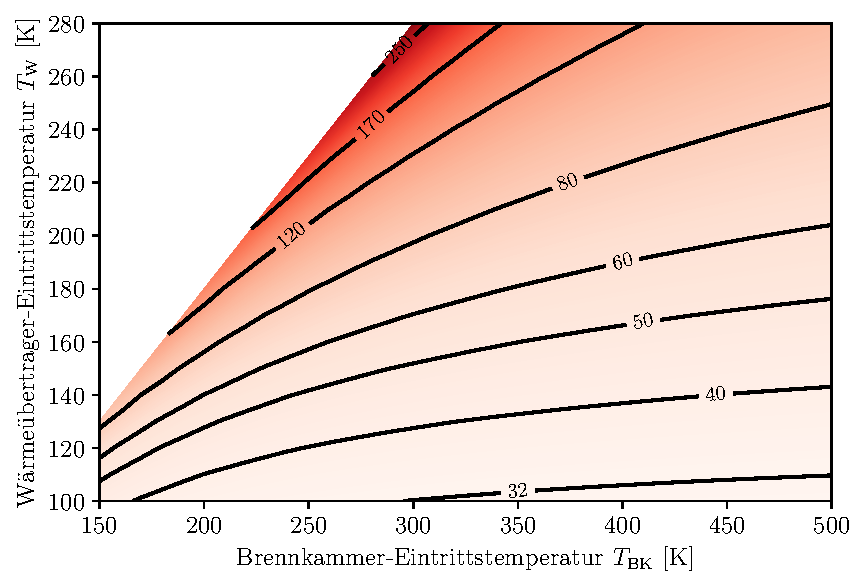
\includegraphics[width=0.9\linewidth]{4_Abbildungen/2_Hauptteil/Ergebnisse/Pumpepowercontour.pdf}
  \caption{Leistungsbedarf Wasserstoff-Kraftstoffsystem mit Pumpe [kW]}
  \label{fig:pumppower}
\end{figure}
\FloatBarrier

Der Gesamtleistungsbedarf steigt mit zunehmender Wärmeübertrager-Eintrittstemperatur, da die geringe Differenz zur Brennkammer-Eintrittstemperatur einen größeren Rezirkulations-Massenstrom erfordert, was die Leistung des Rezirkulationsverdichters erhöht. Zwar führen höhere Brennkammer-Eintrittstemperaturen zu einer Zunahme der spezifischen Arbeit des Rezirkulationsverdichters, jedoch wird dieser Effekt durch den aufgrund der erhöhten Temperaturdifferenz reduzierten rezirkulierten Massenstrom mehr als ausgeglichen. Die Leistung der Hochdruckpumpe ist hingegen unabhängig von den Eintrittstemperaturen (Abbildung \ref{fig:pumpsplit}). 

\begin{figure}[ht]
\centering
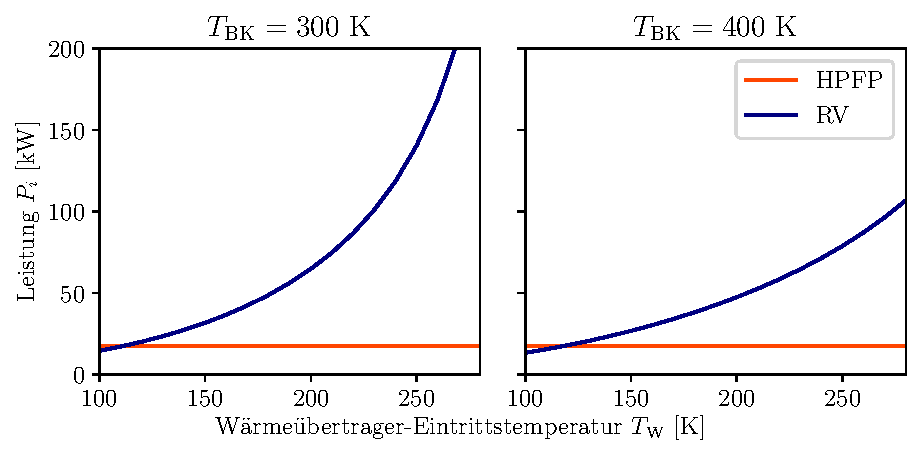
\includegraphics[width=0.9\linewidth]{4_Abbildungen/2_Hauptteil/Ergebnisse/Pumpe_powersplit.pdf}
  \caption{Leistungsaufteilung Architektur mit Pumpe}
  \label{fig:pumpsplit}
\end{figure}
\FloatBarrier

Der Wärmebedarf ist insbesondere mit der Brennkammer-Eintrittstemperatur korreliert. Da die Leistung des Rezirkulationsverdichters mit steigender Wärmeübertrager-Eintrittstemperatur beziehungsweise geringer Differenz der Eintrittstemperaturen zunimmt, liegt in diesem Fall ein verringerter Wärmebedarf vor. Dieses Verhalten ist in Abbildung \ref{fig:pumpheat} dargestellt.

\begin{figure}[ht]
\centering
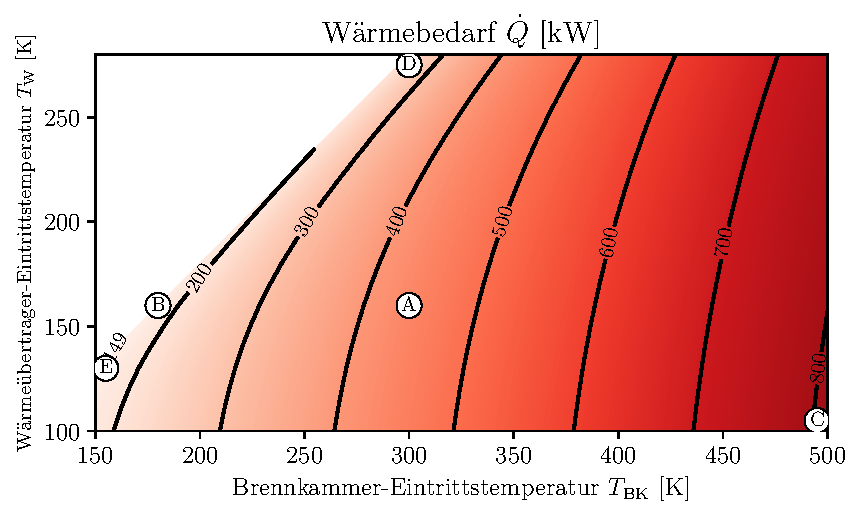
\includegraphics[width=0.9\linewidth]{4_Abbildungen/2_Hauptteil/Ergebnisse/Pumpeheatcontour.pdf}
  \caption{Wärmebedarf Wasserstoff-Kraftstoffsystem mit Pumpe [kW]}
  \label{fig:pumpheat}
\end{figure}
\FloatBarrier

Abbildung \ref{fig:pumpfuel} zeigt den Kraftstoffverbrauch des Triebwerks mit dem Kraftstoffsystem mit Pumpe für die unterschiedlichen Eintrittstemperaturen.

\begin{figure}[ht]
\centering
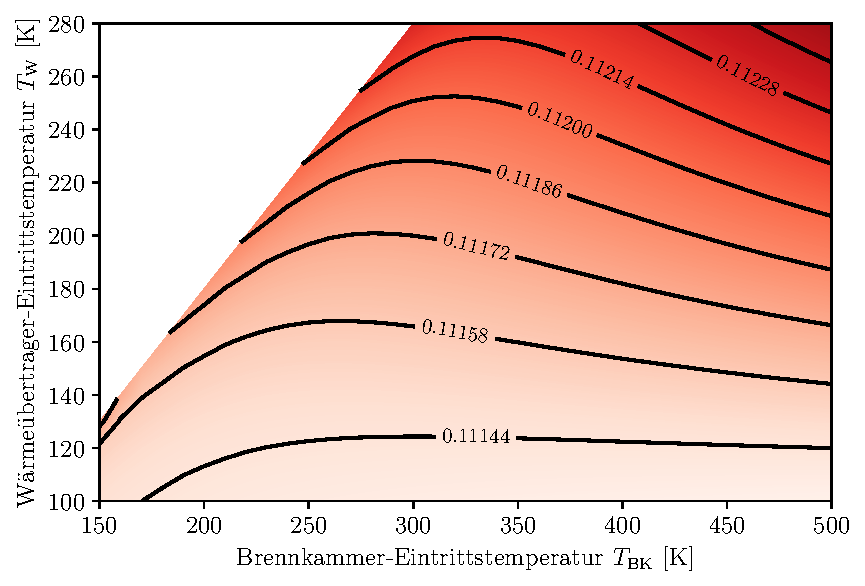
\includegraphics[width=0.9\linewidth]{4_Abbildungen/2_Hauptteil/Ergebnisse/Pumpemassflowcontour.pdf}
  \caption{Kraftstoffverbrauch Wasserstoff-Kraftstoffsystem mit Pumpe [kg/s]}
  \label{fig:pumpfuel}
\end{figure}
\FloatBarrier

Die Leistung des Rezirkulationsverdichters bei hohen Wärmeübertrager-Eintritts-temperaturen verringert den Gesamtwirkungsgrad des Triebwerks. Im Gegensatz dazu hat die Brennkammer-Eintrittstemperatur einen geringeren Einfluss auf den Verbrauch.


\subsection{Vergleich der Wasserstoff-Kraftstoffsysteme}

Im Folgenden werden die Ergebnisse der Parameterstudie für die verschiedenen Wasserstoff-Kraftstoffsysteme miteinander verglichen. Abbildung \ref{fig:comp_power} zeigt den Leistungsbedarf der Kraftstoffsysteme in Abhängigkeit der Wärmeübertrager-Eintrittstemperatur für zwei verschiedene Brennkammer-Eintrittstemperaturen.

\begin{figure}[ht]
\centering
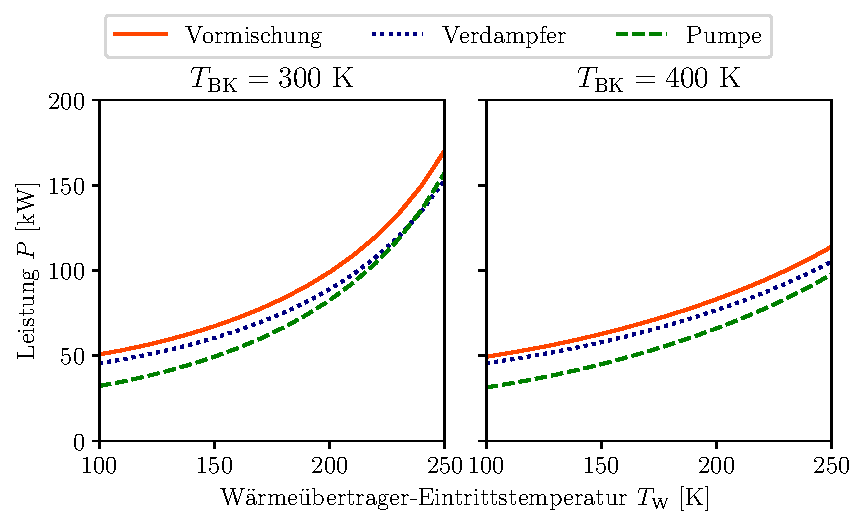
\includegraphics[width=0.9\linewidth]{4_Abbildungen/2_Hauptteil/Ergebnisse/summary_power.pdf}
  \caption{Leistungsbedarf Wasserstoff-Kraftstoffsysteme}
  \label{fig:comp_power}
\end{figure}
\FloatBarrier

Aufgrund der höheren spezifischen Arbeit der Verdichtung im gasförmigen Zustand weisen beide Verdichterarchitekturen im Vergleich zur Pumpenarchitektur einen erhöhten Leistungsbedarf auf. Da die Verdichter des Kraftstoffsystems mit Vormischung bei identischer spezifischer Arbeit einen größeren Massenstrom  fördern als die Verdichter der Architektur mit Verdampfer, hat das Kraftstoffsystem mit Vormischung einen höheren Leistungsbedarf. Dieser Effekt wird bei höheren Brennkammer-Eintrittstemperaturen abgeschwächt, da die Verdampfung in diesem Fall einen geringeren Massenstrom erfordert. Abbildung \ref{fig:comp_split} zeigt den Einfluss der Wärmeübertrager-Eintrittstemperatur auf die Komponenten-Leistungen.

\begin{figure}[ht]
\centering
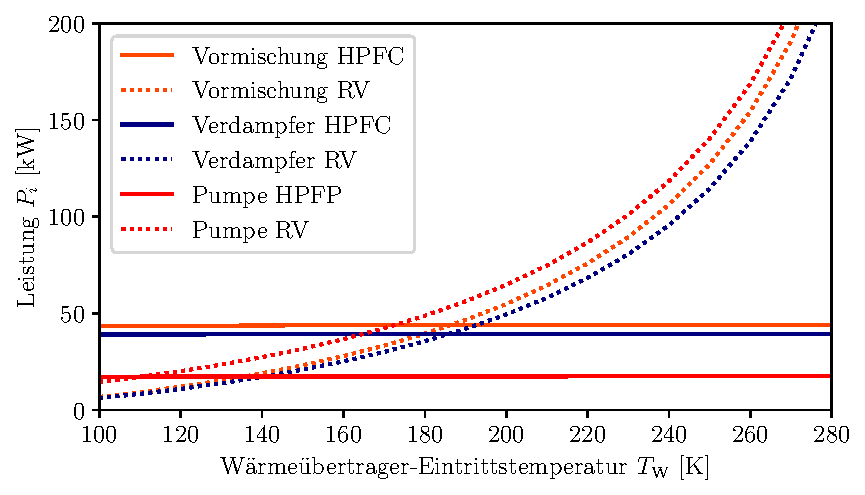
\includegraphics[width=0.9\linewidth]{4_Abbildungen/2_Hauptteil/Ergebnisse/300summary_powersplit.pdf}
  \caption{Leistungsaufteilung Vergleich [$T_\mathrm{BK}=$ \SI{300}{\K}]}
  \label{fig:comp_split}
\end{figure}
\FloatBarrier

Analog zur Architektur mit Pumpe hat die Wärmeübertrager-Eintrittstemperatur bei den Verdichterarchitekturen keinen Einfluss auf die Leistung des Hochdruckverdichters. Da die Verdichterarchitekturen im Vergleich zur Pumpenarchitektur einen geringeren Rezirkulationsmassenstrom aufweisen, fällt auch die Leistung des Rezirkulationsverdichters geringer aus. Abbildung \ref{fig:tbk_split} zeigt den Einfluss der Brennkammer-Eintrittstemperatur auf die Komponenten-Leistungen.

\begin{figure}[ht]
\centering
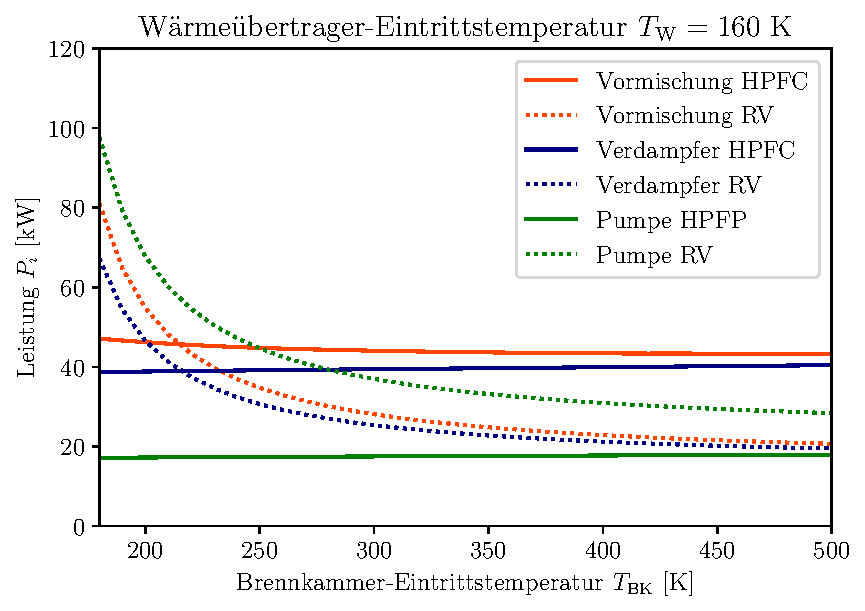
\includegraphics[width=0.7\linewidth]{4_Abbildungen/2_Hauptteil/Ergebnisse/tbkcomp.pdf}
  \caption{Leistungsaufteilung Vergleich [$T_\mathrm{W}=$ \SI{160}{\K}]}
  \label{fig:tbk_split}
\end{figure}
\FloatBarrier

Der Trend sinkender Leistung des Rezirkulationsverdichters bei höherer Differenz der Eintrittstemperaturen setzt sich auch bei den Verdichterarchitekturen fort. Im Gegensatz zu den anderen Architekturen führen steigende Brennkammer-Eintrittstemperaturen bei der Architektur mit Vormischung jedoch zu einer geringfügigen Reduzierung der Leistung des Hochdruckverdichters. Dies ist auf den geringeren erforderlichen Massenstrom für die Verdampfung zurückzuführen. 

Abbildung \ref{fig:stackplot} gibt einen Überblick der Leistungsanteile der Wasserstoff-Kraftstoffsysteme. In der linken Spalte sind die Leistungsanteile in Abhängigkeit der Brennkammereintritts-Temperatur bei konstanter Wärmeübertrager-Eintrittstemperatur dargestellt. Die mittlere Spalte zeigt die Leistungsanteile in Abhängigkeit der Brennkammer-Eintrittstemperatur, aber mit konstanter Temperaturdifferenz. Die rechte Spalte zeigt die Leistungsanteile in Abhängigkeit der Wärmeübertrager-Temperatur bei konstanter Brennkammereintritts-Eintrittstemperatur.

\begin{figure}[ht]
\centering
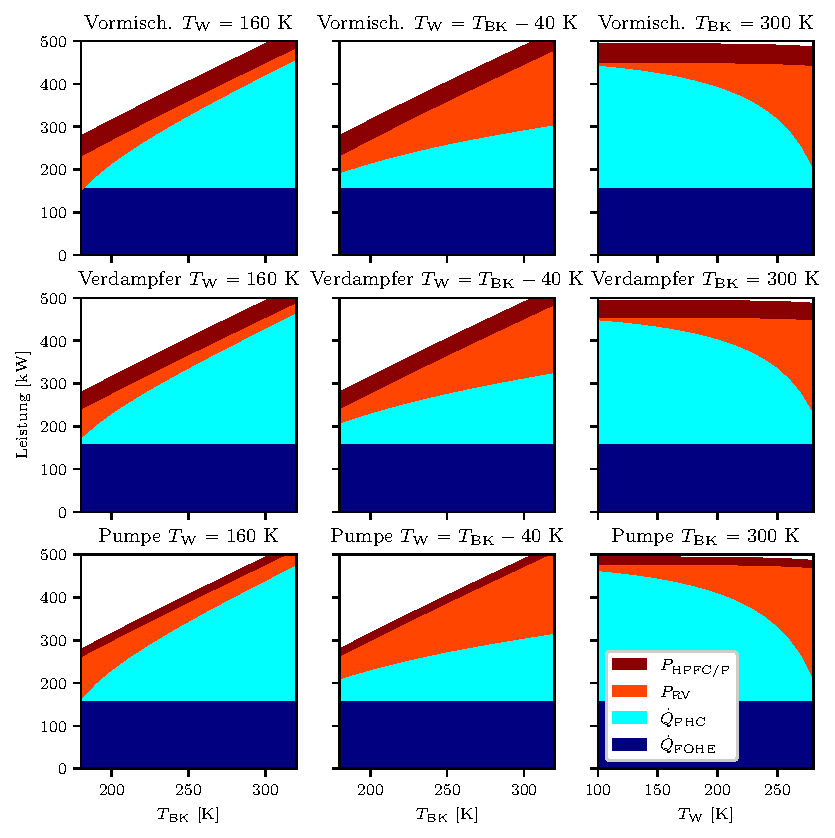
\includegraphics[width=1\linewidth]{4_Abbildungen/2_Hauptteil/Ergebnisse/stackplot_summary.pdf}
  \caption{Stapeldiagramme der Leistungsanteile}
  \label{fig:stackplot}
\end{figure}
\FloatBarrier

Diese Abbildung verdeutlicht den Einfluss der Differenz der Eintrittstemperaturen. Bei einer konstanten Temperaturdifferenz von $T_{BK}-T_W=$ \SI{40}{\K} (mittlere Spalte) liegen die Leistung des Rezirkulationsverdichters $P_{RV}$ und die Wärme der parallelen Wasserstoffverbrennung $\dot{Q}_{PHC}$ über die untersuchten Brennkammer-Eintrittstemperaturen betragsmäßig in einem ähnlichen Bereich. Im Gegensatz dazu nimmt bei konstanter Brennkammer-Eintrittstemperatur der Leistungsanteil des Rezirkulationsverdichters mit steigender Wärmeübertrager-Eintrittstemperatur zu (rechte Spalte).

Eine direkte Empfehlung spezifischer Eintrittstemperaturen lässt sich aus diesen Daten nicht ableiten. Grundsätzlich gilt, dass eine möglichst niedrige hinnehmbare Wärmeübertrager-Eintrittstemperatur den Kraftstoffverbrauch reduziert. Für die Brennkammer-Eintrittstemperatur lässt sich hingegen keine eindeutige Aussage treffen, sodass sie in Abhängigkeit von der Wärmeübertrager-Eintrittstemperatur gewählt werden sollte.

\section{Vergleich Kerosin- und Wasserstoff-Kraftstoffsysteme}

Im Folgenden werden die Wasserstoff-Kraftstoffsysteme mit dem Referenzkraftstoffsystem verglichen. Abbildung \ref{fig:refcomp} zeigt den Betriebsmittelbedarf der verschiedenen Kraftstoffsysteme. Für die Wasserstoff-Kraftstoffsysteme gilt eine Brennkammer-Eintrittstemperatur von $T_\mathrm{BK}=$ \SI{300}{\K} und eine Wärmeübertrager-Eintrittstemperatur von $T_\mathrm{W}=$ \SI{160}{\K}.

\begin{figure}[ht]
\centering
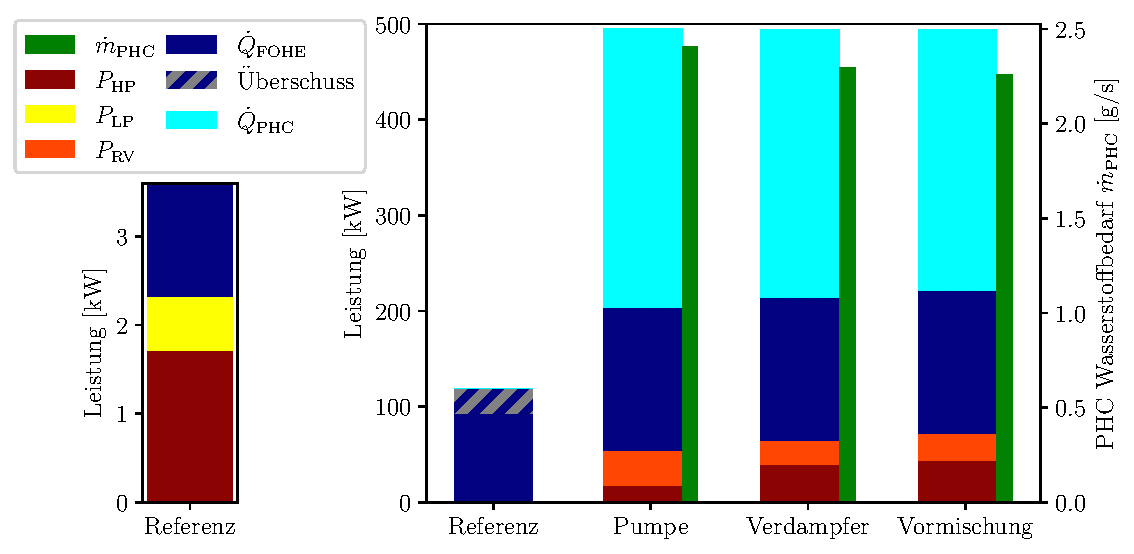
\includegraphics[width=1\linewidth]{4_Abbildungen/2_Hauptteil/Ergebnisse/refcomp.pdf}
  \caption{Betriebsmittelbedarf der Kraftstoffsysteme}
  \label{fig:refcomp}
\end{figure}
\FloatBarrier

Der Betriebsmittelbedarf der Wasserstoff-Kraftstoffsysteme übersteigt den Bedarf des Referenzkraftstoffsystems um einen Faktor von drei. Im Vergleich zum Referenzkraftstoffsystem erfordert das Wasserstoff-Kraftstoffsystem mit Pumpe 22,7-Mal mehr Leistungsentnahme von der Hochdruckwelle und hat einen Wärmefehlbetrag von \SI{278}{\kilo\W}, der durch die parallele Wasserstoffverbrennung gedeckt wird. Bei dem Kraftstoffsystem mit Verdampfer wird sogar das 27,1-Fache an Leistungsentnahme benötigt bei einem Wärmefehlbetrag von \SI{268}{\kilo\W}. Bei dem Kraftstoffsystem mit Vormischung wird das 30,2-Fache an Leistungsentnahme benötigt bei einem Wärmefehlbetrag von nur noch \SI{261}{\kilo\W}. 

Um die Vergleichbarkeit des Kraftstoffverbrauchs sicherzustellen, wird der Energieverbrauch als Produkt aus dem Kraftstoffverbrauch und dem unteren Heizwert bei Normaldruck und einer Temperatur von \SI{298.15}{\K} berechnet.
Abbildung \ref{fig:refenergy} zeigt die Differenz des Energieverbrauchs der Wasserstoff-Kraftstoffsysteme zum Referenzkraftstoffsystem. 

\begin{figure}[ht]
\centering
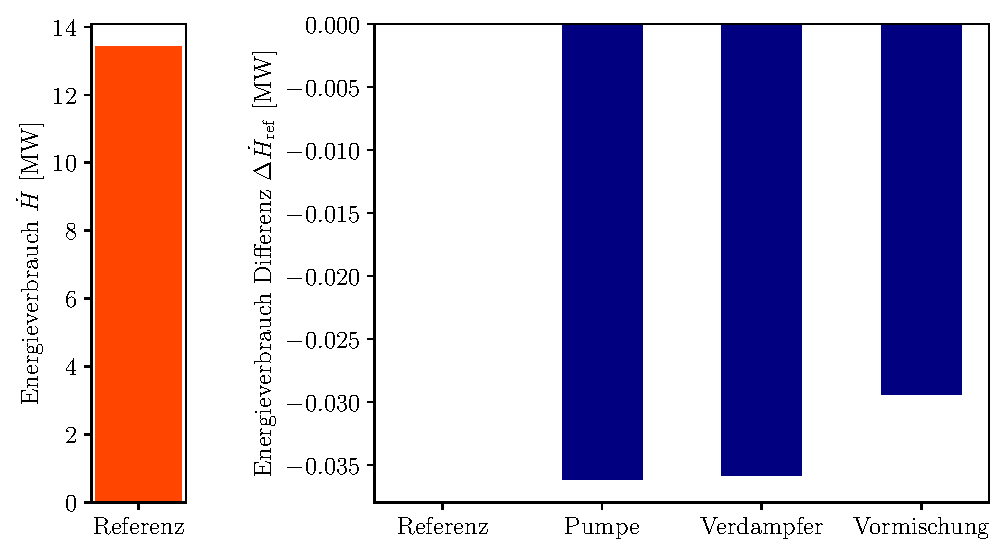
\includegraphics[width=1\linewidth]{4_Abbildungen/2_Hauptteil/Ergebnisse/refenergy.pdf}
  \caption{Energieverbrauch der Kraftstoffsysteme}
  \label{fig:refenergy}
\end{figure}
\FloatBarrier

Trotz des zusätzlichen Betriebsmittelbedarfs verbrauchen die Wasserstoff-Kraftstoffsysteme bis zu $0{,}27\,\%$ weniger Energie. Dies ist auf den höheren Wirkungsgrad des Kreisprozesses des wasserstoffbetriebenen Zyklus zurückzuführen, der durch die abweichenden Abgaseigenschaften begünstigt wird.